\section{Simulation Experiments}\label{sec:experiments}
We used the RAPsim  simulator  \cite{rapsim} for the evaluation of our algorithms. RAPsim allows users to simulate microgrid networks (involving main grid, microgrids with solar and wind power generating capabilities, individual homes having solar panels). We implement our models on a network with three microgrids (see Figure~\ref{exp}), out of which two operate on solar and one (in the middle) on wind power. The solar microgrid on the right has more generation capacity than the one on the left. Each microgrid can serve power to homes that are only connected to it. 

%We implemented our models on a network with three microgrids. Two of them  operate on solar renewable generation and the other on wind energy. To simulate the renewable generation, we use RAPsim software \cite{rapsim}. RAPsim is an open source simulator for analyzing the power flow in microgrids. It has a provision for simulating the renewable generation, which is the main feature that we use in our experiments. We construct our microgrid model as shown in Fig 2. We can see that there are three microgrids, two of them operating on the solar energy and the other on the wind energy. The solar microgrid in the right has more capacity than that of the one in the left. These microgrids also have electrical connections from the main grid. Each microgrid provides power to the respective houses on their power line. 

\begin{figure}[thbp]
	\centering
	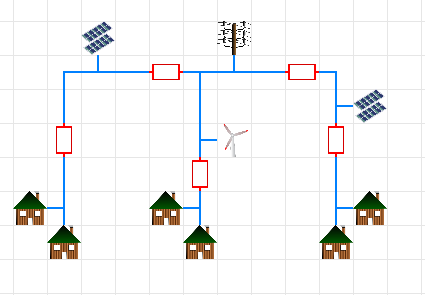
\includegraphics [scale = 0.6]{experimental_setup.jpg}
        \caption{Experimental Setup}
	\label{exp}
\end{figure}
\subsection{Implementation}
We implement our \textbf{ADL-sharing model} described in section \ref{sec:model}. For comparison purposes, we also implement the following models.\footnote{The implementation is available at \url{https://github.com/saikotireddy/PES-GM---Smart-Grid/archive/master.zip}.} 
\begin{itemize}
	\item \textbf{Greedy-ADL model}: In this model, microgrids exhibit greedy behavior. They share power only after filling their respective batteries fully. The action $u_t^i$ at each time instant $t$ is bounded as follows:  
	\begin{align}
	-min(M_t^i, & B_t^i - nd_t^i + \max_{1\leq j \leq 2^n} A_t^i(j) ) \leq u_t^i \nonumber\\ &\leq max(0, nd_t^i - B_t^i).
	\end{align}
	Thus, if $ nd_t^i < 0$, decision is taken on the amount of power to buy in order to satisfy the demand and to fill the battery. If $ nd_t^i > 0$, then it is first used to fill the battery fully and if any excess power is left, it will be sold to the other microgrids.
	
	\item \textbf{Non-ADL model}:  In this model, ADL demand is treated as normal demand. Penalty is levied immediately if the demand is not met in the current time slot.
%This model is similar to the $ADL-sharing$ model, but without the concept of ADL jobs. In this model, the ADL demand is included in the main demand. Unlike the $ADL-sharing$ model, there is no flexibility of intelligently scheduling the ADL jobs. 	
\end{itemize}
\subsection{Simulation setup}
We used RAPsim simulator to generate real world per hour renewable energy data for each of the microgrids  for the month of September 2017. We used this data to fit a Poisson distribution for energy generation at each microgrid. The number of decision time periods in a day is taken to be 4. The mean of the Poisson distribution for the two solar and one wind power respectively are as follows :

$$ \left[ \begin{array}{ccccc}
	0 & 0.5410 & 6.5965 & 4.3712 \\
	0 & 0.7350 & 8.6901 & 5.7239 \\
	3.6087 & 3.2167 & 3.1405 & 3.8590
\end{array} \right],$$

where the element $(i,j)$ represents the Poisson mean of microgrid $i$ at time $j$.
For each time period, non-ADL demand ($d_t^i$) at each of the microgrids can be one of the following  three values: 2, 4 and 6 units. The price ($p_t^i$) per unit energy values is considered to be one of 5, 10 and 15. 
% For demand at each microgrid, we considered three values - 2, 4 and 6 units. 
%We simulate the above setup for the month of September 2017 in the RAPsim and collect the wind and solar renewable power generated each day every hour. Using this data, we fit Poisson distribution and obtain the Poisson mean. 
%The parameters for our experiments are described below. The number of decision time periods is taken to be 4 (i.e., t = 4). We consider 3 demand values for all the microgrids - 2, 4 and 6 units. 
The transition probability matrix for non-ADL demand and the Price values are generated randomly.

%\[P_{1}= \left[ \begin{array}{ccc}
%0.2 & 0.6 & 0.2 \\
%0.1 & 0.2 & 0.7 \\
%0.8 & 0.1 & 0.1
%\end{array} \right],
%%
%%P_{2}=
%\left[ \begin{array}{ccc}
%0.2 & 0.2 & 0.6 \\
%0.8 & 0.1 & 0.1 \\
%0.2 & 0.7 & 0.1
%\end{array} \right]
%\]
%
%\[P_{3}= \left[ \begin{array}{ccc}
%0.5 & 0.5 & 0 \\
%0 & 0.5 & 0.5 \\
%1 & 0 & 0
%\end{array} \right],
%%
%Q=
%\left[ \begin{array}{ccc}
%0.2 & 0.4 & 0.4 \\
%0.1 & 0.5 & 0.4 \\
%0.5 & 0.4 & 0.1
%\end{array} \right]
%\]
The maximum size of the battery ($B_t^i$) and maximum power that a microgrid can obtain from the main grid ($M_t^i$) are considered to be 8 and 10 units respectively.
At each microgrid, we consider 3 ADL jobs, $\{\gamma_{1}^{i} =  (1,2), \gamma_{2}^{i} =  (1,3),  \gamma_{3}^{i} =  (2,4)\}$ at the start of the day, where ADL job $\gamma_{j}^{i} =  (a,b)$ requires $a$ units of energy within $b$ time slots. In the $Non-ADL$ model, the ADL demand is added to the demand at $t = 1$ each day. %We considered each day is having three time slots. 
We ran all our models for each of the following $c$ (penalty per unit of unmet demand) values : 0, 5, 10 and 30, respectively.
\subsection{Results}
The algorithms are trained for $10^7$ cycles. We used the average profit obtained by each microgrid as a performance metric to evaluate the models. Figure~\ref{r2} plots the average profit obtained for each microgrid versus the number of iterations, when $c = 10$ for all the three models. 
\begin{figure}[thbp]
	\centering
	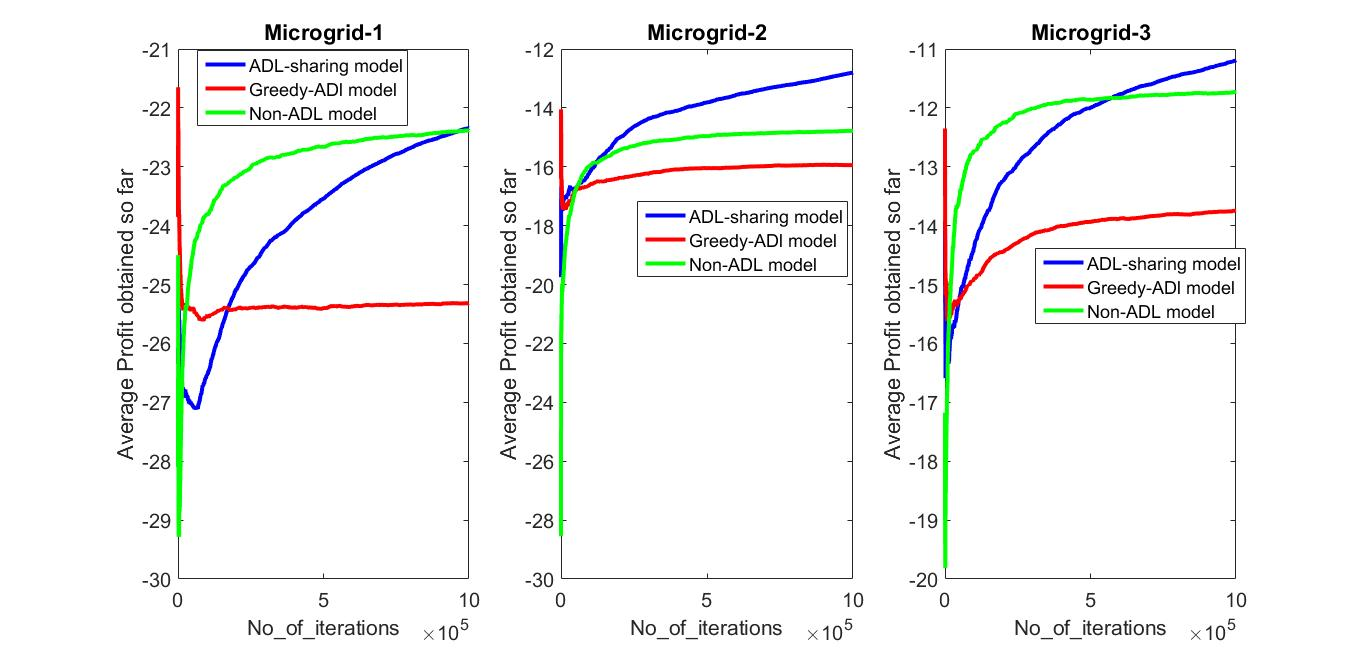
\includegraphics[scale = 0.2]{second_plot.jpg}
	\caption{Average profit metric comparision when $c = 30$ for a three microgrid network.}
        \label{r2}
\end{figure}

Figure~\ref{r1} plots the average profit obtained for each microgrid versus $c$ for all the three models. We run the trained models for 1000 runs to obtain the average reward. 
\begin{figure}[thbp]
	\centering
	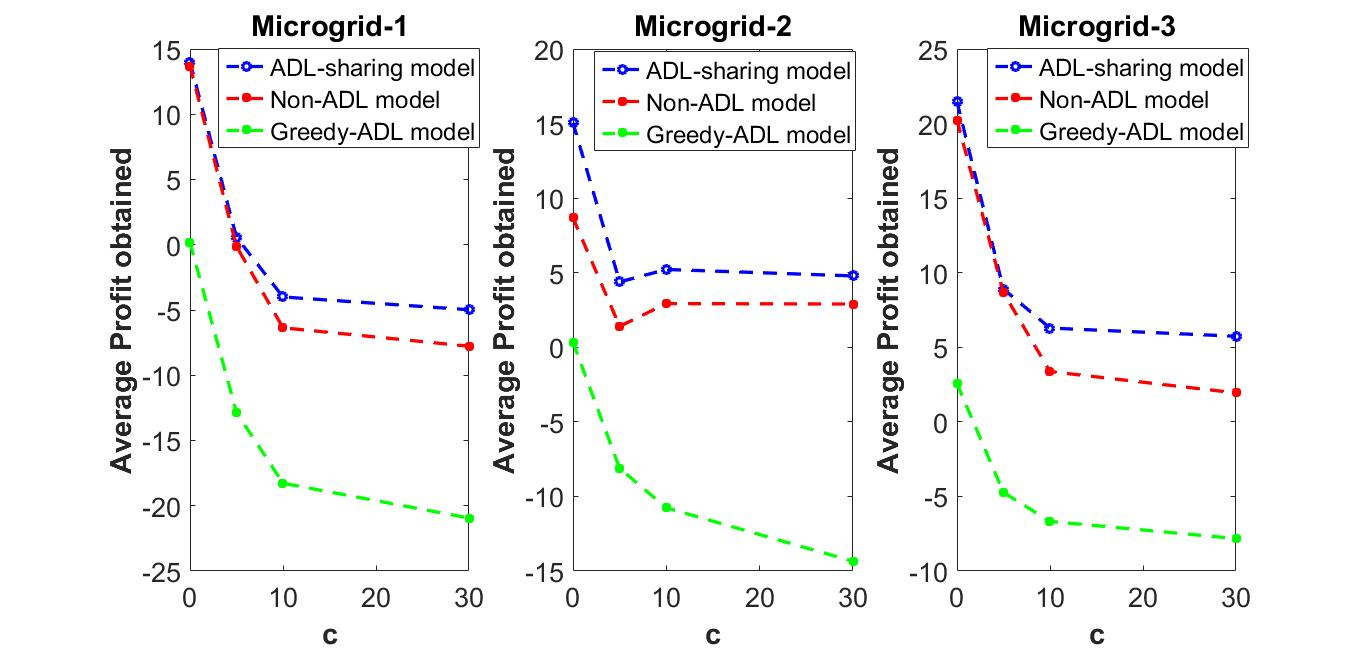
\includegraphics[scale = 0.2]{first_plot.jpg}
	\caption{Average profit metric comparision versus $c$.}
	 \label{r1}
\end{figure}
\subsection{Discussion}

\begin{itemize}

\item In  the $Greedy-ADL$ model there is less buying and selling of power compared to the other models.
%In the $Greedy-ADL$ model the sharing of power is done only after filling the battery. Therefore, even though there is less buying of power in $Greedy-ADL$, there is very little selling of power as well.
 Therefore the overall profit obtained is not high. Thus intelligent sharing of power among microgrids as with the RL technique, yields more profit than in the $Greedy-ADL$ case. 

\item We also observe that, $ADL-sharing$ model outperforms the $Non-ADL$ model. In $ADL-sharing$, there is a flexibility to intelligently schedule the ADL jobs according to the non-ADL demand and price. 
%But in the $Non-ADL$ case, the penalty is immediately levied if the demand (including the ADL demand) is not met. 
Hence we conclude that intelligently scheduling the ADL demand results in better performance.



%From our experiments we make the following observations:
%\begin{itemize}
%\item When $c = 0$, the agents need not buy power to satisfy the excess demand as they don't incur penalty.
 %In the $ADL-sharing$ model, we observe that all the agents fill the battery when the price is low and sells the power when the price is high. %Hence there will be not much sharing among the agents. 
%Hence, the profit obtained is very high compared to the other models. When $c >0$, we observe the sharing among the microgrids. 
% because in $Greedy-ADL$ model, the power bought will be first stored in the battery irrespective of price. 
%In $Non-ADL$ model, the demand values are higher compared to other models and hence there will very less excess power to sell and make profits.
%\item We observed less sharing among the microgrids for the higher values of $c$. It is a desired as the penalty ($c$) is more for unmet demand, microgrids tend to store more in the battery than to share. 
%\item When $c >0$, we observe the sharing  as each microgrid has different configurations of current and future demand and renewable resources. An agent operating on solar renewable generation in the time period 2 share the excess power with the other agents, as it is generates more supply as the day progresses. A the same time, agent operating on wind renewable generation buys the power to store in its battery, if it expects more demand than it generates in future time period. This results in the sharing of power among the agents.   
	
%\item From the above discussion we conclude that our proposed model provides more profits by exhibiting the following intelligent behavior: (a) Schedules few of the ADL jobs at the beginning, few at the end and few at the middle of their allowed execution time window to exploit flexible nature of the ADL demand. (b) microgrids do not sell all of its surplus energy to the other microgrids if there is more demand than supply in the future (particularly, solar microgrids sell excess energy during the midday but not at the end of the day).
%\item In Figure~\ref{r2}, we observe that as the number of iterations increases, the performance of the learning algorithm improves. Moreover, the model 2 and the model 3 converges faster than that of our model 1, because of larger state and action space in model 1. 
\end{itemize}
